%! Author = Adham Aijou
%! Date = 20/02/2023

% Preamble
\documentclass[11pt]{article}
\usepackage{mdframed}
\usepackage[ngerman]{babel}
\usepackage[T1]{fontenc}
\usepackage[utf8]{inputenc}
\usepackage[paper=a4paper,left=40mm,right=20mm,top=25mm,bottom=20mm,footskip=25pt ]{geometry}
\usepackage[backend=biber,style=alphabetic,citestyle=alphabetic-verb]{biblatex}
\usepackage{mathptmx} %Font Times New Roman
\usepackage[toc,nonumberlist]{glossaries} %Erstellt ein Abkürzungsverzeichnis
\usepackage{array}
\usepackage{wrapfig} %Bilder können fließend in den Text eingebunden werden
\usepackage{xcolor}
\usepackage{filecontents}
\usepackage{sectsty}
\usepackage{titletoc}
\usepackage{tocvsec2}
\usepackage[title,titletoc]{appendix}
\usepackage{hyperref}
\usepackage{enumitem}
\usepackage{pgfplots}
\usepackage{tikz}
\usepackage{longtable} % Tabellen können Seitenumbrüche enthalten
\usepackage{listings} % Listings für Codebeispiele
\lstset{basicstyle=\footnotesize,
    inputencoding={utf8},
    extendedchars=false,
    language={Bash},
    escapeinside=``,
    frame = single}
\lstset{literate=%
    {Ö}{{\"O}}1
    {Ä}{{\"A}}1
    {Ü}{{\"U}}1
    {ß}{{\ss}}1
    {ü}{{\"u}}1
    {ä}{{\"a}}1
    {ö}{{\"o}}1
    {~}{{\textasciitilde}}1
}

\lstMakeShortInline[columns=fixed, basicstyle=\ttfamily\color{darkgray}]@

%\addtokomafont{disposition}{\rmfamily} %Serifenschrift für Überschriften
\counterwithout{footnote}{section} %Durchgehende Fußnoten Nummerierung
\setlength\parindent{0pt} % Einrückung für neue Absätze
\usepackage[font=footnotesize,justification = centering]{caption} %Font für Bildunterschriften
\usepackage{pifont}   % Wird für den Punkt neben den Seitzenzahlen benötigt
\usepackage[footsepline=1pt]{scrlayer-scrpage} % Anpassung von Kopf/Fußzeilen
\usepackage{setspace}
\usepackage{microtype}
\usepackage{tabularx}
% Document

\begin{document}
    \makeglossaries
    %! Author = Adham Aijou
%! Date = 20/02/2023

% Preamble
\documentclass[11pt]{article}

% Packages
\usepackage{amsmath}
\usepackage{graphicx}
\pagenumbering{Roman}
\begin{titlepage}
    \centering
%    \includegraphics[width=0.35\textwidth]{bilder/itn.jpg}\par\vspace{1cm}
    \vspace{2cm}
    Fachhochschule für die Wirtschaft Hannover \\
    - FHDW -\\
    {\scshape\Large Praxisarbeit \par}
    \vspace{1cm}
    {\huge\bfseries Ressourcen- und Terminplanung in Office365 mit Hilfe von Microsoft Graph API \par}
    \vspace{3cm}

    \normalsize{
        \begin{tabular}{l l}
            \textbf{Adham:} & \textbf{Aijou} \\
            &	Brinker Straße 72 \\
            &	30851, Langenhagen \\
            \\

            \textbf{Mentor:} & \textbf{Prof. Dr.  Ing. Klinger}\\
            \\
            \textbf{Studiengruppe:} & \textbf{HFI421IN}\\
            \\
            \textbf{Matrikelnummer:}  & \textbf{600142} \\
            \\
            \textbf{Ausbildungsbetrieb:}  & \textbf{DOOH media GmbH}\\
            & Frankenring 18\\
            & 30855 Langenhagen    \\
            \\
            \textbf{Eingereicht am:} & xx.xx.xxxx
        \end{tabular}\\
    }
    \vfill
%    \flushright \includegraphics[width=0.35\textwidth]{bilder/doohmediaLogo.png}\par\vspace{1cm}

\end{titlepage}
% Document
\begin{document}



\end{document}
    %! Author = mboehme
%! Date = 21.02.2023



% Document
    \tableofcontents
    \newpage



    %! Author = mboehme
%! Date = 21.02.2023

% Preamble

% Document

\section{Einleitung}\label{sec:einleitung}
Die Praxisarbeit befasst sich mit der Ressourcen- und Terminplanung in Office365 mithilfe von Microsoft Graph API~\cite{microsoftGraphApi}.
Die Arbeit ist in drei Teile gegliedert.
Im ersten Teil wird die Theorie der Ressourcen- und Terminplanung in Office365 mithilfe von Microsoft Graph API erläutert.
Im zweiten Teil wird die praktische Umsetzung der Theorie beschrieben.
Im dritten Teil wird die Arbeit abschließend bewertet.
    \newline
    \subsection{Fragestellungen der Arbeit}\label{subsec:fragestellungen-der-arbeit}
Die Fragestellungen der Arbeit lauten:
    \begin{itemize}
        \item Wie funktioniert die Ressourcen- und Terminplanung in Office365 mithilfe von Microsoft Graph API?
        \item Wie kann die Ressourcen- und Terminplanung in Office365 mithilfe von Microsoft Graph API praktisch umgesetzt werden?
        \item Wie kann die Arbeit abschließend bewertet werden?
    \end{itemize}
Konkret bedeutet dies:
\newline
Inwiefern und wie sinnvoll, ist der Einsatz von Microsoft Graph API für die Ressourcen- und Terminplanung in Office365, im Vergleich zu anderen APIs.
Dabei sollte berücksichtigt werden, dass dies auf den Kundenauftrag bezogen ist.
Wie sollte sowas umgesetzt werden und welche Aspekte der Microsoft Graph API sind dafür relevant?
Letztenendes soll herausgefunden werden, wie man die Arbeit quantitativ und qualitativ bewerten kann.
    \subsection{Ziele der Arbeit}\label{subsec:ziele-der-arbeit}
Die Ziele der Arbeit sind wie folgt:
    \begin{itemize}
        \item Die Theorie der Ressourcen- und Terminplanung in Office365 mithilfe von Microsoft Graph API zu erläutern.
        \item Die praktische Umsetzung der Theorie anhand eines Kundenauftrags zu beschreiben.
        \item Die Arbeit abschließend zu bewerten.
    \end{itemize}
Für die Ziele bedeutet dies, dass die Fragestellungen der Arbeit beantwortet werden müssen.
Sowohl die Theorie als auch die praktische Umsetzung der Theorie, müssen in der Arbeit beschrieben werden.
Es muss immer wieder auf die Kundenanforderungen zurückgegriffen werden.

    \subsection{Ergebnisse der Arbeit}\label{subsec:ergebnisse-der-arbeit}
Die Arbeit hat alle Ziele erreicht.
    \newglossaryentry{SPA}{name=Single Page Application (SPA), description={Eine Single Page Application (SPA) ist eine Webanwendung, die nur eine HTML-Seite besitzt.
    Diese Seite wird beim Laden der Anwendung geladen und bleibt während der gesamten Nutzung der Anwendung bestehen.}, first={Single Page Application (SPA)}, text={SPA}, short=SPA}
%\newglossaryentry{SPA}{name=SPA, description={Eine Single Page Application (SPA) ist eine Webanwendung, die nur eine HTML-Seite besitzt.}}
%\newacronym{SPA}{SPA}{Single Page Application}
    Die Microsoft Graph API ist erfolgreich eingesetzt und die Ressourcen- und Terminplanung in Office365, mithilfe von der Microsoft Graph API, wurde erfolgreich als~\gls{SPA} umgesetzt.
\newglossaryentry{TBT}{name={Total-Blocking-Time (TBT)}, description= {Die Total-Blocking-Time (TBT) ist eine Metrik, die die Gesamtzeit misst, die eine Seite blockiert wird, bis sie interaktiv ist.},
first={Total-Blocking-Time (TBT)}, text={TBT}}

Die detaillierten Aspekte Ergebnisse der Arbeit sind in den Kapiteln~\ref{sec:ergebnis} und ~\ref{sec:technische-umsetzung} beschrieben.
Das ausformulierte Ergebnis und die Schlussfolgerung dieser, sind in Kapitel~\ref{sec:ergebnis} erläutert.
\newpage


    %! Author = Adham Aijou
%! Date = 23.02.2023
\subsection{Use Case}
\begin{tabularx}{\textwidth}[b]{|l*{2}{|X}|}\hline
    \caption{Use Case - Terminbuchung}
    \label{tab:Terminbuchung}
    Use Case & Ressourcen- und Terminplanung in Office365 mit Hilfe von Microsoft Graph API\\

    Titel & Finde freie Termine in einem Kalender für eine bestimmte Ressource\\
    \hline
    Beschreibung & Der Benutzer möchte einen Termin in einem Kalender für eine bestimmte Ressource finden.\\
    \hline
    Akteure & Benutzer, Ressource, Kalender\\
    \hline
    Vorbedingungen & Der Benutzer ist angemeldet.\\
    \hline
    Nachbedingungen & Der Benutzer hat einen Termin in einem Kalender für eine bestimmte Ressource gefunden und/oder hat einen Termin gebucht.\\
    \hline
    Normaler Ablauf & \begin{enumerate}
        \item Der Benutzer geht zu einem Tablet, welcher vor dem Raum angebracht wurde, welcher die Ressource stellvertretend repräsentieren soll.
        \item Der Benutzer sieht die verfügbaren Zeiten für die Ressource und den jetzigen Status der Ressource.
        \item Der Benutzer wählt einen Termin aus.
        \item Der Benutzer bucht den Termin.
        \item Der Benutzer erhält eine Bestätigung oder eine Fehlermeldung.
    \end{enumerate}\\
    \hline
\end{tabularx}
    %! Author = Adham Aijou
%! Date = 23.02.2023

\subsection{Systemschnittstellen}\label{subsec:systemschnittstellen}
%first column is too wide, make everything fit into one A4 page
\begin{tabularx}{\textwidth\footnotesize}{|l*{2}{|X}|} \hline
%    \multicolumn{2}{|c|}{\textbf{Microsoft Graph API}}\\
    \caption{Termin buchen}
    \label{tab:TerminBuchen}
 Kurzbeschreibung: & Im UI kann der User sich mit der Ressource einloggen, die für die Zukunft als Repräsentant für die reelle Ressource (z.B einen Raum) gelten soll.
    Dann gilt dieser User immer als Teilnehmer der Buchungen und kann in seinen verfügbaren Zeiten gebucht werden.
    Der User kann zudem andere Mitarbeiter hinzufügen, um sie einerseits über das Meeting zu informieren und andererseits, um automatisch überprüfen zu können, wann alle am besten Zeit haben.
    Darauf basierend werden dem User verfügbare timeslots zur Buchung angezeigt.
    Auch die Dauer des Termins soll einstellbar sein.
    Es gibt zudem einen optionalen Betreff für den Termin.
    Der gebuchte Termin reflektiert sich dann im UI in der Liste der für den Tag schon gebuchten Termine, für die Ressource.
    Zudem soll der Nutzer sehen können ob innerhalb der nächsten 30 Minuten ein Termin für die Ressource ansteht oder ob einer schon am Passieren ist, anhand einer farblichen UI .

    REST API Anfragen werden dann an die Microsoft Graph API geschickt, um diese Wünsche zu kommunizieren.\\
    \hline
    Akteure: & Mitarbeiter\\
    \hline
    Häufigkeit: & Variablel pro Ressource, Firma und Anzahl Ressourcen\\
    \hline
    Komplexität: & Mittlere bis hohe Komplexität\\
    \hline
    Vorbedingungen: & \begin{enumerate}
                          \item User muss eingeloggt sein (Nutzerdaten können nicht gesehen oder eingespeichert werden) und Zugriffsrechte akzeptieren.
                          \item Optionale Teilnehmer
                          \item Termindauer
                          \item Verfügbare Termine
                          \item Terminbetreff
                          \item Zeitzone
                          \item Für die Microsoft Graph API kommt noch der Access Token / Client ID von unserer Azure App zur Authentifizierung dazu
    \end{enumerate}\\
    \hline
    Ausgaben: & \begin{enumerate}
                    \item Buchung erfolgreich oder nicht
                    \item Neue verfügbare Termine
                    \item Der neue Termin wird in der Liste der gebuchten Termine angezeigt
                    \item Falls die Buchung nicht geklappt haben sollte, wird der User darüber informiert
    \end{enumerate}\\
    \hline
    Use Case: &~\ref{tab:Terminbuchung}\\
    \hline
Schnittstellen: & \begin{enumerate}
                        \item Microsoft Graph API
                        \item User Interface
                        \item Backend
                      \end{enumerate}\\
    \hline
    Aufgerufene Aktionen: & Notwendige: \begin{enumerate}
                                        \item Termin buchen
                                        \item Termin finden
                                            \end{enumerate}
            \linebreak Optionale: \begin{enumerate}
                                      \item Teilnehmer hinzufügen
                                      \item Terminbetreff hinzufügen/ändern
                                        \item Termindauer ändern
                                      \end{enumerate}\\
    \hline
\end{tabularx}
\pagebreak
    %! Author = mboehme
%! Date = 21.02.2023



% Document
\section{Theorie}\label{sec:theorie}

\subsection{Microsoft Graph API}\label{subsec:microsoft-graph-api}
Die Microsoft Graph API ist eine \gls{RESTful} web API, die es einem erlaubt auf Daten von Microsoft 365 und Office 365 zuzugreifen.
\newglossaryentry{RESTful}{
    name=RESTful,
    description={RESTful ist ein Synonym für Representational State Transfer. RESTful ist ein Architekturstil für die Entwicklung von Webdiensten.}
}
Mit Hilfe dieser API wurde das Projekt letztendlich umgesetzt.
Weitere standen jedoch zur Verfügung:
\begin{itemize}
    \item Microsoft Outlook API
    \item Microsoft Exchange API
    \item Microsoft SharePoint API
    \item Microsoft OneDrive API
    \item Microsoft Teams API
    \item Microsoft Power Automate
\end{itemize}
Einige dieser APIs, sind nur für bestimmte Microsoft 365 und Office 365 Abonnements verfügbar.
Die Microsoft Graph API ist jedoch für alle Abonnements verfügbar.
Zudem ist die Microsoft Graph API die einzige API, die es einem erlaubt auf alle Daten von Microsoft 365 und Office 365 zuzugreifen, da sie die meisten anderen APIs integriert.
Der wichtigste Faktor bei der Entscheidung war es jedoch, dass die Microsoft Graph API, mithilfe von Azure AD, die Authentifizierung und Autorisierung von Benutzern erlaubt. Dies ist für die Anwendung von großer Bedeutung, da es dem Benutzer ermöglicht sich mit seinem Microsoft 365 oder Office 365 Account anzumelden und somit auf seine Daten zuzugreifen.


    \input{istZustand}
    %! Author = Adham Aijou
%! Date = 22/02/2023

% Preamble
\pagebreak
\section{Vorgehensweise}\label{sec:vorgehensweise}

\subsection{Prototyp}\label{subsec:prototyp}
Erst wurde ein Prototyp mithilfe von vuejs entwickelt, basierend auf folgendem Mockup, welcher erstellt wurde bevor die Grafikdesigner ein Konzept erstellt hatten:
%Das ist Vorschlag 1. Muss in Soll-Zustand geändert werden
\par\vspace{1cm}
    \centering
    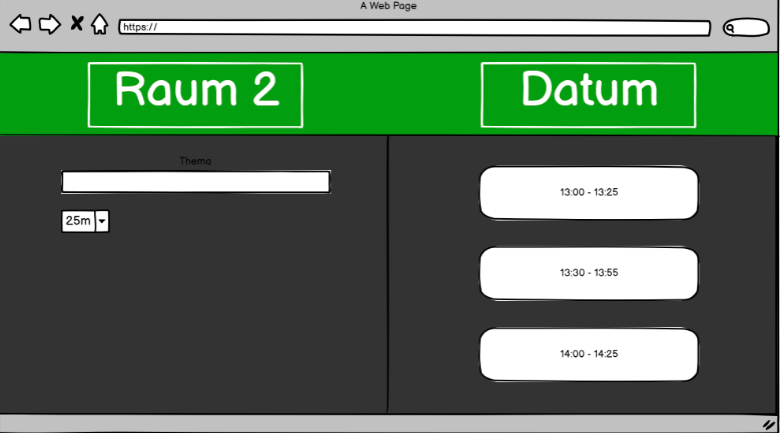
\includegraphics[width=0.8\textwidth]{Bilder/mockup}
    \caption{Mockup}
    \label{fig:Mockup}
\par\vspace{1cm}
\raggedright
    %! Author = mboehme
%! Date = 23.02.2023

\subsection{Technische Umsetzung}\label{subsec:technische-umsetzung}

\subsubsection{Grobe Planung}
Das Ganze wird als eine Azure App deployt.
Diese lässt localhost Verbindungen zu und gibt einem die Möglichkeit das ganze als Single Page Application zu entwickeln, mit einem lokalen cookie cache für den eingeloggten Account.
Somit ist keine Individualisierung notwendig.
\newline
Es wird, lokal, mithilfe von Dory-node.js gehostet.
Diese lässt localhost Verbindungen zu und gibt einem die Möglichkeit die Web-Applikation wird als Single-Page-Application, mit einem lokalen cookie cache für den eingeloggten Account, entwickelt.
Somit ist keine Individualisierung notwendig.
Zudem kann dann mit dem Phillips Display die Web-Applikation aufgerufen werden und als eine Art Model eines Model-View-Controllers verwendet werden.
\newline
Der Player braucht auf der OMS den Content-Typen \("\)Web\("\) mit der URL: \("\)http://localhost:3000/content\("\).
Diese Seite wird dann lokal vom Player aufgerufen, worauf der Dory-nodejs Server antwortet und die tatsächliche Seite anbietet, die lokal auf dem Display liegt.
So ist die URL durchgehend, auf allen Geräten, identisch, damit die OAuth 2.0 URI Bedingungen ~\cite{OAuth-2.0-Simplified} erfüllt sind.
Durch den Verzicht auf einen Webserver werden kosten eingespart, da Updates eher selten passieren sollten.
\newline
Zudem ist es für die Sicherheit der Nutzer so viel besser, da wir deshalb keinen Zugriff auf ihre Daten haben.
Zeiten müssen, bei jeglichen API Anfragen an die Microsoft Graph API, ISO 8601 Konform sein \@.
Dies ist wichtig, da Zeitzonen des Nutzers, ungleich der Zeitzonen der Server, sein können.
Außerdem können Sommer- und Winterzeiten unterschiedlich sein, was zu Problemen führen kann.
Es muss also bei der Datenverarbeitung darauf geachtet werden, dass die Zeiten immer ISO 8601 Konform sind, aber bei der Anzeige, kann man die Zeiten in die Zeitzone des Nutzers umrechnen.
Beispielsweise, im Terminbuchungsmenü, muss dem Nutzer die Zeit angezeigt werden, die lokal für ihn gilt.
Sobald dieser Termin aber gebucht wird, muss die Zeit in die Zeitzone des Servers umgerechnet werden, damit die Buchung auch dort korrekt verarbeitet wird.
\newline
\pagebreak
\subsubsection{Benutzte Hardware und Software}
Hardware:
\begin{itemize}
    \item Philips 10BDL4551T/00 (Firmware: FB01.13, SICP Version: v.2.05)
\end{itemize}
\newline
Die Hardware ist ein Philips~\cite{10BDL4551T/00} Display.
Dieses Display ist ein 10 Zoll (ca. 25 cm) Touchscreen.
Es hat eine Auflösung von 1280x800 Pixeln und benutzt Android.
Dieses Display ist für Digital Signage gedacht und kann so auch als solches verwendet werden.
\newglossaryentry{SICP}{name=SICP, description={SICP steht für Serial (Ethernet) Interface Communication Protocol.
SICP ist ein Protokoll, das es ermöglicht, mit dem Display, an der OS vorbei, zu kommunizieren.}}
Die eingebauten RGB LED Strips können per~\gls{SICP} angesteuert werden.
Dafür braucht wird Dory-Node.js genutzt, um auf einen lokalen Server zu hören und die Anfragen an das Display weiterzuleiten.
Es wird dafür keine Internetverbindung benötigt, da kein Websocket benötigt wird.
Die Details der SICP Daten sind öffentlich schwierig zu finden, aber im Internet sind einige Beispiele zu finden.
Befehle werden in Hexadezimal geschrieben und an das Display gesendet.
Die Verschlüsselung passiert, indem ein XOR aller vorausgehenden Bytes genommen und als checksum mitgegeben wird.
\newline
\newline
Software:
\begin{itemize}
    \item Vue.js 3.x
    \item Microsoft Graph API per NPM Package
    \item Dory-Node.js
    \item Azure App
    \item Babel
    \item Webpack
    \item Node.js
    \item NPM
    \item Git
    \item EsLint
    \item IntelliJ IDEA
\end{itemize}
\newline
Vue.js ist ein JavaScript Framework und transpiliert die Vue.js Dateien in JavaScript, damit sie von jedem Browser ausgeführt werden können.
Es ist darauf spezialisiert, Single Page Applikationen zu entwickeln.
\newline
\newline
Dory-Node.js ist ein Node.js Server, der es ermöglicht, eine Web-Applikation lokal zu hosten.
Dies wird benötigt, um einerseits die Raumbuchungsseite lokal anzubieten, damit die absoluten Redirect-URI Bedingungen von Microsoft und oAuth 2.0 erfüllt werden können und andererseits, um die Anwendung auf dem Display zu hosten und als Schnittstelle zwischen der Seite und dem den LED-Strips des Displays zu agieren.
\newline
\newline
Die Microsoft Graph API wird per NPM Package verwendet, um die Anfragen an die Microsoft Graph API zu vereinfachen und den User einzuloggen.
\newline
\newline
Babel ist ein JavaScript Compiler, der es ermöglicht, moderne JavaScript Features zu verwenden, die von älteren Browsern nicht unterstützt werden, um so die Kompatibilität zu erhöhen.
\newline
\newline
Webpack ist ein JavaScript Bundler, der es ermöglicht, mehrere JavaScript Dateien zu einer einzigen zusammenzufassen, um so die Ladezeiten zu verkürzen.
\newline
\newline
Node.js ist ein JavaScript Runtime, der es ermöglicht, JavaScript Code auszuführen, ohne einen Browser zu benötigen.
Es ist das sogenannte Backend dieser Anwendung.
Dieser wird per Dory-Node.js gehostet.
\newline
\newline
NPM ist ein Package Manager, der es ermöglicht, JavaScript Packages zu installieren und zu verwalten.
\newline
\newline
Git ist ein Versionskontrollsystem, welches es ermöglicht, Änderungen an Dateien zu verfolgen und zu verwalten.
Dies wurde aber in Zusammenhang mit GitLab verwendet, da dies der derzeitige, etablierte Standard der DooH media GmbH ist.
\newline
\newline
EsLint ist ein Linter, der es ermöglicht, JavaScript Code zu analysieren und zu formatieren.
Da Testfälle bei JavaScript Projekten nicht immer vollständig möglich sind, ist es wichtig, dass der Code einheitlich ist und keine Fehler enthält.
Deshalb achtet EsLint auf die Einhaltung von Regeln, damit erst gar keine Fehler entstehen, die der JavaScript Compiler nicht erkennen kann.
Beispielsweise wird überprüft, ob Variablen deklariert wurden, bevor sie verwendet werden und anders herum.
\newline
\newline
IntelliJ IDEA ist eine IDE, die es unter anderem ermöglicht, JavaScript Code zu schreiben und zu debuggen.
\newline
\newline

\subsubsection{Weiterentwicklung der groben Planung}
Es wurde eine Azure App erstellt, die die Authentifizierung der Anwendung und des Users übernimmt.
\newline
Dort wird der User eingeloggt und die Anwendung leitet ihn auf die Seite weiter, die er vorher besucht hat, welche in diesem Fall, die Raumbuchungsseite ist.
\newline
Es wurde jede Woche Rücksprache mit dem Kunden gehalten, um die Anforderungen zu besprechen und zu erfüllen.
Aber auch intern wurde Rücksprache gehalten, was denn sinnvoll ist und was nicht.
\newline
So wurde jede Woche die Anwendung weiterentwickelt und verbessert.
Teilweise wurden auch neue Features hinzugefügt, die nicht im Pflichtenheft standen, aber sinnvoll waren.
Manche Features wurden auch wieder entfernt, da sie nicht sinnvoll waren oder von anderen Features abgedeckt wurden.
\newline
%Ablauf der Entwicklung
\newline
\subsubsection{Ablauf der Entwicklung}
Nachdem der erste Prototyp fertig war und Rücksprache gehalten wurde, wurde angefangen die Anwendung zu entwickeln.
Design und Funktionalität wurden dabei partiell parallel entwickelt, wobei die Funktionalität immer Priorität hatte.
Über 95 Commits wurden die Änderungen an der Anwendung festgehalten.
\newline
Es wurde ein Testgerät benötigt, um die Anwendung zu testen.
Ein Phillips 10BDL4551T/00 Display wurde dafür an die Wand gehängt und mit dem Internet verbunden.
Zudem wurde es so eingerichtet, wie es auch beim Kunden laufen soll.
\newline
Es wurde täglich aktiv genutzt, um so Fehler zu finden und Feedback zu geben.
Das Feedback wurde dann, falls sinnvoll, in die Anwendung eingearbeitet.
Solche praktischen Tests sind sehr wichtig, um Intuitivität und Benutzerfreundlichkeit zu gewährleisten.
Es war einerseits hilfreich, um vorgesehene Abläufe zu testen, andererseits aber auch um Fehler zu finden, die nicht vorgesehen waren, indem Monkey Testing~\cite{Monkey-Testing-Book1} betrieben wird.
\newline
\subsubsection{Rest-Anfragen}
Mithilfe der oDatav4 (~\cite{oData}) API wurden die Daten aus der jeweiligen Microsoft Datenbank im Voraus gefiltert, um so nicht notwendige Daten zu vermeiden und Performance drastisch zu erhöhen, als auch Datenvolumen zu sparen.
Die Daten wurden dabei in JSON Format zurückgegeben.
Die oData v4 API verhält sich dabei wie eine SQL Datenbank, wobei die Daten in Tabellen gespeichert sind.
Es wurden die Klauseln \("\$\)filter\("\) und \("\$\)top\("\) verwendet, um nur Termine für den aktuellen Tag und nächsten Tag zu erhalten und dies einzuschränken auf die top 300 Termine, falls jemand versucht das System zu überlasten.
Eine Sortierung ist nicht notwendig, da die Termine bereits nach Startzeit sortiert sind.
Hier sieht man die oData v4 API Anfrage:
\newline
%add javascript code formatting
\begin{lstlisting}[language=javascript,label={lst:JavaScript oData v4 API Anfrage}]
     let url =  "https://graph.microsoft.com/v1.0/me/findMeetingTimes/?$filter=start/dateTime" +  "ge"  + "${todayDate} and end/dateTime le ${tomorrowDate}&$top=300";
\end{lstlisting}
\newline
Es wurden im Voraus, Befehle im Microsoft Graph Explorer~\cite{Microsoft-Graph-Explorer} ausgeführt, um zu testen, ob die Anfrage funktioniert und ob die Daten in der gewünschten Form zurückgegeben werden.
Jedoch hat sich herausgestellt, dass der Microsoft Graph Explorer nicht korrekt funktioniert und teilweise Befehle nicht entgegennimmt, die laut Microsoft Dokumentation funktionieren sollten.
Evident ist dies, da die Anwendung korrekt funktioniert und die REST API Anfragen korrekt funktionieren und auch im Request-Response Zyklus keine Fehler auftreten.
\newline
\newline
Falls die Anfrage nicht funktioniert, wird eine Fehlermeldung angezeigt, die den User darauf hinweist, dass die Verbindung zum Server derzeit unterbrochen ist.
Wie Fehlermeldungen behandelt werden sollten, findet man im folgenden Buch: ~\cite{interaction-design-book1}.
Fehlermeldungen sollten immer so gestaltet sein, dass sie den User nicht verunsichern, sondern ihn auf die Lösung des Problems hinweisen.
Auch bei der Gestaltung der Fehlermeldung sollte darauf geachtet werden, dass sie nicht zu lang ist, da der User sonst nicht mehr weiß, was er tun soll.
Bei Kiosk Anwendungen ist es besonders wichtig, dass die Fehlermeldungen kurz und prägnant sind, da der User ohnehin in einer Situation ist, in der er wahrscheinlich nicht viel Zeit hat.
Genaueres dazu, befindet sich, im genannten Buch, unter dem Kapitel \("Errors, Alerts, and Confirmation"\) und unter dem Kapitel \("Platform and Posture - Designing for kiosks"\).
Das bedeutet, dass Fehler, die dazu führen, dass die Anwendung nicht mehr funktioniert, groß und auffällig dargestellt werden sollten, damit der User sie nicht übersehen kann und versteht, dass er die Anwendung nicht mehr nutzen kann, bis das Problem behoben wurde.
Andererseits sollten Fehler, die nicht dazu führen, dass die Anwendung nicht mehr funktioniert, klein und unauffällig dargestellt werden, damit der User nicht gestört wird.
Es liegt nicht in der Verantwortung des Nutzers, dass die Anwendung nicht funktioniert, sondern in der Verantwortung des Entwicklers, solange es um die lokale Verarbeitung geht.
\newline
\subsubsection{Timer}
Der Timer, welcher die übrig bleibende Zeit bis zum nächsten Termin anzeigt funktioniert, wie folgt:
\newline
\newline
Es wird die Zeit bis zum Ende den jetzigen Termin berechnet, ausgehend von der Zeit, die zum Anfang des jetzigen Termins vergangen ist, und in Millisekunden umgerechnet.
Dann wird eine sich drehende Animation erstellt, die für diese Dauer abläuft.
\newline
Da die Dauer angepasst werden kann, muss bei Datenänderungen die Animation neu berechnet werden.
Damit dies nicht ohne Grund passiert, wird geprüft, ob die Dauer sich geändert hat.
Die Daten dafür werden im Local Storage gespeichert.
Falls eine Änderung stattgefunden hat, wird die Animation neu berechnet.
Bei der Änderung werden, damit die Animation visuell nicht von vorne anfängt, die Animationsdauer und die vergangene Zeit als neue Animationsdauer aufaddiert und die vergangene Zeit als negative Animationsverzögerung gesetzt, damit die Animation visuell betrachtet dort ist, wo sie relativ zur neuen Dauer sein sollte.
\newline
\newline
Die Formel lautet, wie folgt:
\newline
\newline
\begin{equation}
\begin{aligned}
    \text{Vergangene Zeit} &= \text{Jetzt} - \text{Start} \\
\text{Animationsdauer} &= \text{Ende} - \text{Start} \\
    \text {Animationsverzögerung} &= \text{-Vergangene Zeit} \\
\end{aligned}
\end{equation}
\newline
\newline
Man kann die Formel verkürzen und die Animationsdauer und -verzögerung direkt berechnen, aber es ist verständlicher, falls jemand in der Zukunft dies nachvollziehen möchte.
\newline
\newline
Hier sieht man den zugehörigen JavaScript Code:
\newline
\newline
\begin{lstlisting}[language=javascript,label={lst:JavaScript Timer}]
let currentEventBeginningTime = localStorage.getItem('currentEventBeginningTime');
let timePassed = (new Date() - new Date(currentEventBeginningTime + 'Z')) / 1000;
let animationDuration = ((new Date(currentEventEndTime + 'Z') - new Date(currentEventBeginningTime + 'Z')) / 1000);
firstHandSpan.style.animationDuration = animationDuration  + 's';
secondHandSpan.style.animationDuration = animationDuration + 's';
firstHandSpan.style.animationDelay = -timePassed + 's';
secondHandSpan.style.animationDelay = -timePassed  + 's';
\end{lstlisting}
\newline
\newline
Um die Animation während ihrer Laufzeit zu ändern, wird ein sogenannter Reflow ~\footcite{JavaScriptAnimationsReflow} erzwungen, indem die offsetWidth Eigenschaft abgefragt, die Animationsdauer und -verzögerung neu gesetzt und der Animationsname erst entfernt und dann wieder hinzugefügt wird.
\newline
\newline
\subsubsection{Persistente Datenspeicherung}
Um die Daten der Anwendung zu speichern, wurde für kleinere Datensätze der Local Storage verwendet.
Dieser ist in jedem Browser verfügbar und darf bis zu 5 MB groß sein.
\newline
\newline
Für größere Datensätze wurde IndexedDB~\cite{IndexedDB} verwendet.
\newglossaryentry{caniuse}{name={caniuse.com},description={Caniuse is a website that shows you browser support for various features and includes references to the relevant specifications.}}
Dies ist eine NoSQL Datenbank, die in jedem gängigen Browser~\cite{caniuse-indexedDB} (\gls{caniuse}) verfügbar ist.
Die maximale Größe bei Chrome beträgt 80\(\%\) des verfügbaren Speichers.
Da es im Internet viele, sich widersprechende Angaben zu dieser Größe gibt, wurde diese manuell, mit folgendem Code, in der Konsole des Browsers, getestet:
\newline
\newline
\begin{lstlisting}[language=javascript,label={lst:JavaScript IndexedDB Speichergröße}]
    if (navigator.storage && navigator.storage.estimate) {
    const quota = await navigator.storage.estimate();
    // quota.usage -> Number of bytes used.
    // quota.quota -> Maximum number of bytes available.
    const percentageUsed = (quota.usage / quota.quota) * 100;
    console.log("You've used ${percentageUsed}% of the available storage.");
    const remaining = quota.quota - quota.usage;
    console.log("You can write up to ${remaining} more bytes.");
    }
\end{lstlisting}
\newline
\newline
Die Festplatte, auf der dies getestet wurde, hatte ca. 828 GB freien Speicher.
Das Ergebnis lautete wie folgt:
\newline
\newline
\begin{lstlisting}[language=javascript,label={lst:JavaScript IndexedDB Speichergröße Ergebnis}]
    You've used 0.000002393592594674544% of the available storage.
    You can write up to 599726105785 more bytes.
\end{lstlisting}
\newline
\newline
%equation
\begin{equation}
    \begin{aligned}
       \text{verbleibender Speicher} &= \text{599726105785 Bytes}\\
       \newline
       \text{599726105785 Bytes} \text{ * 10}\textsuperscript{-9} &= \text{599,726105785 Gigabytes}\\
        \newline
        \newline
    \end{aligned}
\end{equation}
\newline
\newline
Das sind etwas über 70 \%\) der verfügbaren Speicherkapazität.
Hier ist davon auszugehen, dass die restlichen 10 \%\) für andere Daten schon verwendet werden.
Zudem ist zu betrachten, dass die \"\).\"\) Schreibweise für Dezimalzahlen in JavaScript verwendet wurde, während wiederum die \"\),\"\) Schreibweise für die mathematische Gleichung verwendet wurde.
Dies hat den Hintergrund, dass die \"\),\"\) Schreibweise in JavaScript nicht grundsätzlich unterstützt wird, beziehungsweise, die Konvention beim Programmieren verlangt, dass man auf Englisch programmiert und im Englischen die Dezimalzahlen mit einem Punkt geschrieben werden.
\newline
\newline
Die Datenbank befindet sich aufgrund ihrer geringen Komplexität in der 5. Normalform.
Der Schlüssel besteht aus dem Namen der Firma, zu der, das Logo gehört und gibt das nicht Primärattribut zurück, welches das Bild, in Base64, enthält.
Schlüssel müssen eindeutig sein.
IndexedDB unterstützt die Eigenschaft \"\)unique\"\), welche dafür sorgt, dass der Schlüssel eindeutig ist.
Jedoch gehen wir auch manuell noch einmal sicher, dass der Schlüssel eindeutig ist, also dass sich dieser, noch nicht in der Datenbank befindet.
Eine weitere Aufteilung würde zu Informationsverlust führen, da der Firmenname eindeutig ist.
\newline
\newline
Zwar gibt es die Möglichkeit die Bilder für Firmen, zu updaten, welcher der User auch so wahrnimmt, jedoch wird der Schlüssel des alten Bildes entfernt und ein neuer Schlüssel mit dem neuen Bild hinzugefügt.
Dies ist notwendig, da der Schlüssel eindeutig sein muss.
Somit löschen wir den alten Eintrag und fügen einen neuen hinzu.
Unabhängig von der Interaktion mit der Datenbank, wird sichergestellt, dass sinnfreie Anfragen an die Datenbank nicht gesendet werden.
Falls der User beispielsweise ein Bild hochlädt, welches bereits in der Datenbank, für genau den gleichen Schlüssel, vorhanden ist, wird die Anfrage an die Datenbank nicht gesendet oder falls der User versucht ein Bild aus der Datenbank zu entfernen, welches gar nicht existiert.
\newline
\newline

%    \bibliography{main}
%    \bibliographystyle{plain}
    \printglossaries
\end{document}
